\documentclass[a4paper,10pt]{article}

\usepackage[utf8]{inputenc}
\usepackage[margin=1.2cm]{geometry}
\usepackage{graphicx}
\usepackage{amsmath}
\usepackage{amsfonts}
\usepackage{amssymb}
\usepackage{hyperref}
\usepackage{listings}
\usepackage{xcolor}
\usepackage{caption}
\usepackage{subcaption}
\usepackage{float}
\usepackage{booktabs}
\usepackage{multirow}
\usepackage{array}
\usepackage{tabularx}
\usepackage{lipsum}

\definecolor{codegreen}{rgb}{0,0.6,0}
\definecolor{codegray}{rgb}{0.5,0.5,0.5}
\definecolor{codepurple}{rgb}{0.58,0,0.82}
\definecolor{backcolour}{rgb}{0.95,0.95,0.92}

\lstdefinestyle{mystyle}{
    backgroundcolor=\color{backcolour},   
    commentstyle=\color{codegreen},
    keywordstyle=\color{magenta},
    numberstyle=\tiny\color{codegray},
    stringstyle=\color{codepurple},
    basicstyle=\ttfamily\footnotesize,
    breakatwhitespace=false,         
    breaklines=true,                 
    captionpos=b,                    
    keepspaces=true,                 
    numbers=left,                    
    numbersep=5pt,                  
    showspaces=false,                
    showstringspaces=false,
    showtabs=false,                  
    tabsize=2
}

\lstset{style=mystyle}

\newcommand*\ttvar[1]{\texttt{\expandafter\dottvar\detokenize{#1}\relax}}
\newcommand*\dottvar[1]{\ifx\relax#1\else
  \expandafter\ifx\string_#1\string_\allowbreak\else#1\fi
  \expandafter\dottvar\fi}


\setlength{\parindent}{0pt}

\title{\textbf{WiFi Traffic Classification Report}}
\author{Luca Moriondo}
\date{A.A. 2024/2025}

\begin{document}
\pagenumbering{gobble}
\begin{center}
    \Large\textbf{WiFi Traffic Classification Report}\\
    \large{Luca Moriondo}\\
\end{center}

\textit{This document is a report extracted from the WiFi Traffic Classification project GitHub page. For more information, please refer to the project's GitHub repository at \href{https://github.com/MorioSnek/wifi-traffic-classification}{this link}}.

\subsection*{Capture Processing}
I personally found it easier to convert the whole Wireshark capture file into a format that can be processed by pandas easily, in particular \texttt{.csv}. To do so, it's possible to use the tshark command-line tool that comes with Wireshark. The following command can be used to filter data and copy various information from a \texttt{.pcap} or \texttt{.pcapng} file to a \texttt{.csv}:

\begin{lstlisting}[language=bash]
tshark -r ./private/capture.pcapng \
  -Y "wlan.addr == XX:XX:XX:XX:XX:XX && wlan.fc.type=2" \
  -T fields -E header=y -E separator=, -E quote=d \
  -e frame.time_epoch \
  -e frame.len \
  -e wlan.sa -e wlan.da -e wlan.ta -e wlan.ra \
  -e wlan.fc.type -e wlan.fc.subtype \
  -e wlan.fc.pwrmgt \
  -e radiotap.dbm_antsignal \
  -e wlan.qos.priority \
  -e wlan_radio.snr \
> ./private/traffic.csv
\end{lstlisting}

\subsection*{Classical Analysis}
The first part of this project focuses on classical traffic analysis without machine learning.\\
The script src/plots.py processes the CSV exported with tshark and computes several statistical features of Wi-Fi traffic for a given station MAC address.\\

Specifically, the script:
\begin{itemize}
    \item Splits the traffic into fixed-size time windows (default: 15 seconds).
    \item Separates uplink and downlink packets.
    \item Computes per-window features.
    \item Extracts the Power Management bit to determine when the station is in sleep or awake mode, highlighting sleep periods in the plots.
    \item Produces time-series plots of all the above features, saved as .png images in the data/ folder.
\end{itemize}

This step provides a feature extraction and visualization pipeline that will serve as the foundation for the next stage, where machine learning techniques will be applied to classify user activities from encrypted Wi-Fi traffic.

\subsection*{Machine Learning Approach}
The machine learning side was developed using the scikit-learn library Random Forest. In particular, its functioning is based on the following steps:
\begin{itemize}
    \item \textbf{\textit{Feature extraction:}} the relevant features are extracted from the raw traffic data, contained in \ttvar{model/features_W15.csv}.
    \item \textbf{\textit{Data labeling:}} the labels are assigned to the features based on the type of activity. This is done manually via the script \ttvar{srclabeling.py}, which generates the files \ttvar{model/labels_by_time_W15.csv} and \ttvar{model/features_labeled_W15.csv}.
    \item The dataset is split into training and test sets (based on the parameter TEST SIZE), a Random Forest classifier is trained on the training portion, and its performance is evaluated on the test set through accuracy, classification report, and confusion matrix.
\end{itemize}

\subsection*{Results}
\subsubsection*{Signal strength}
For the first part, the plots generated provide initial insight regarding the RSSI and the SNR, just to be sure that the test is mostly valid. As plotted, the RSSI and the SNR are not only in the expected range, but also strictly correlated. This highlights the absence of noise during this experiment.
\begin{center}
    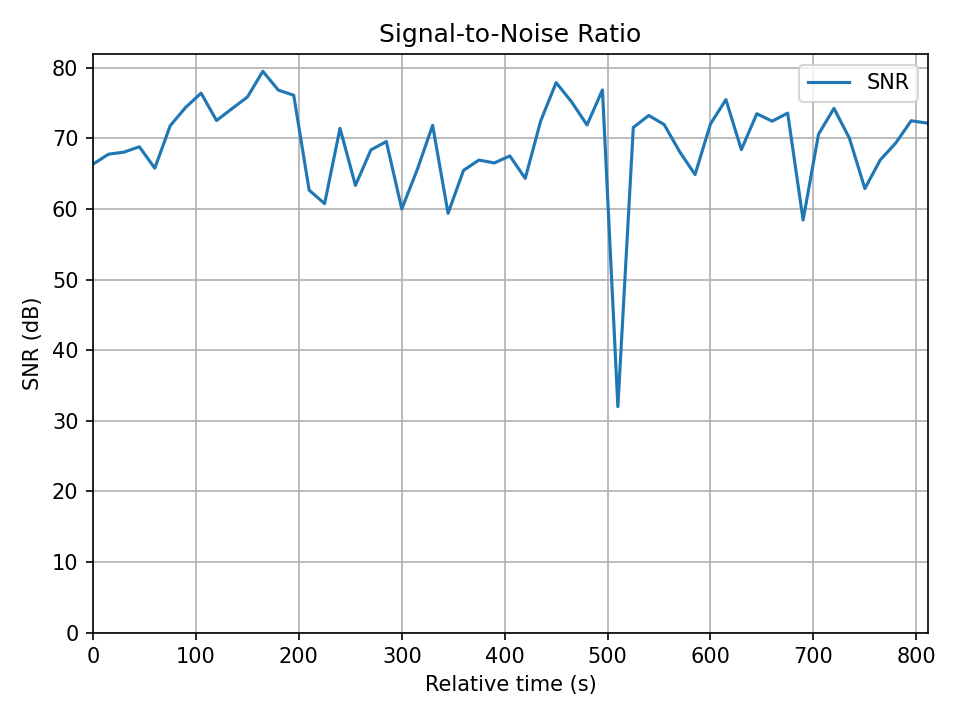
\includegraphics[width=.4\textwidth]{img/plot_snr_W15.png}
    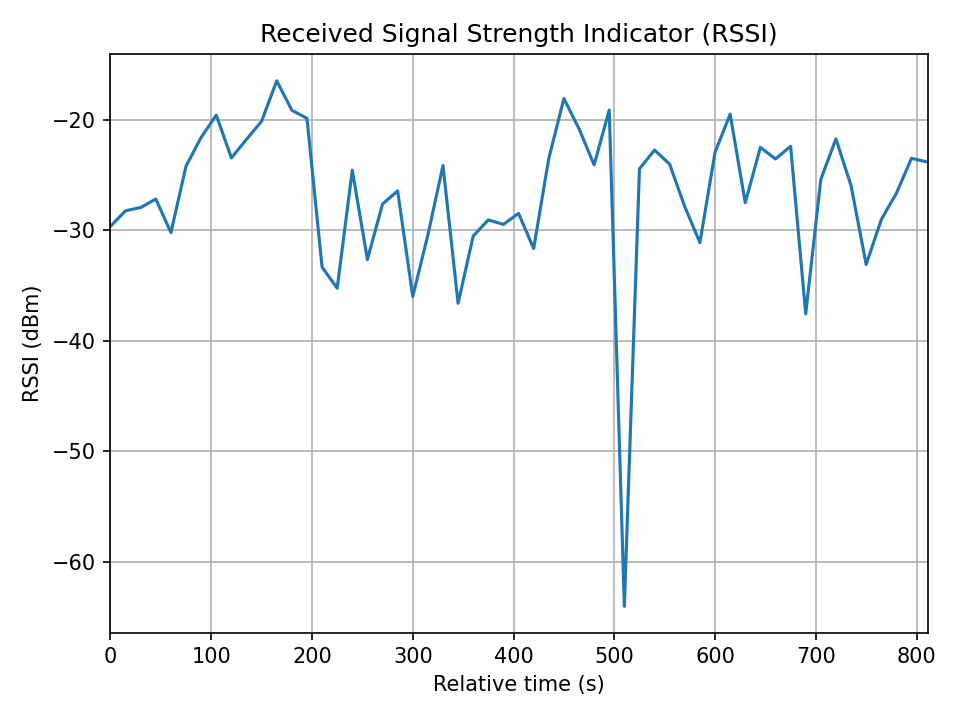
\includegraphics[width=.4\textwidth]{img/plot_rssi_W15.png}
\end{center}

\subsubsection*{Throughput and Frames per second}
The plots regarding the frames captured all highlight in red the areas where the station transceiver was off most of the time.
\begin{center}
    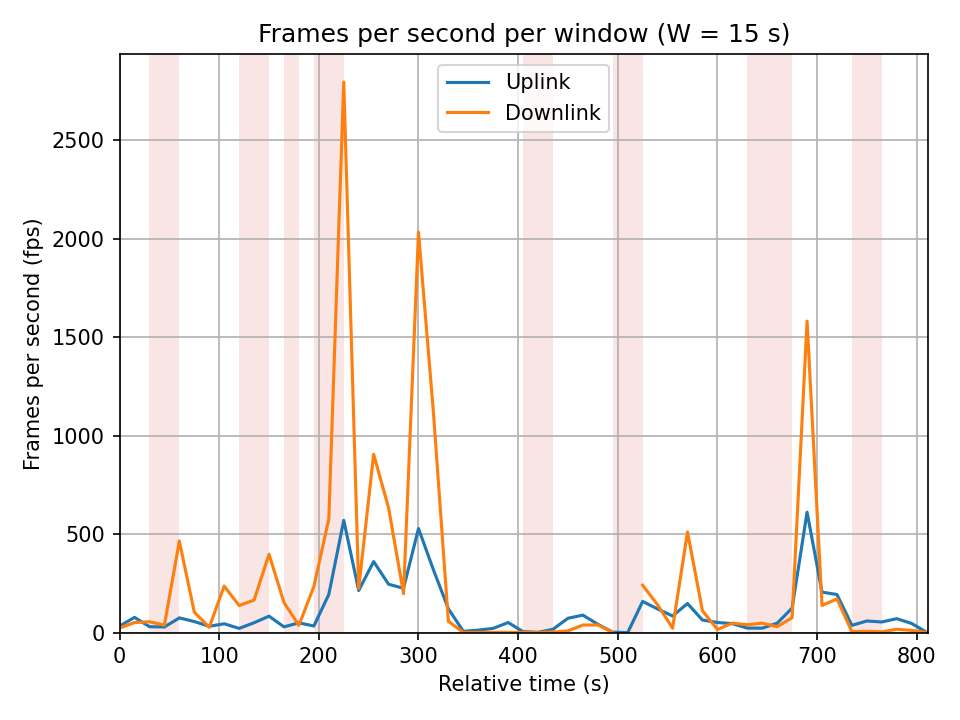
\includegraphics[width=.3\textwidth]{img/plot_fps_W15.png}
    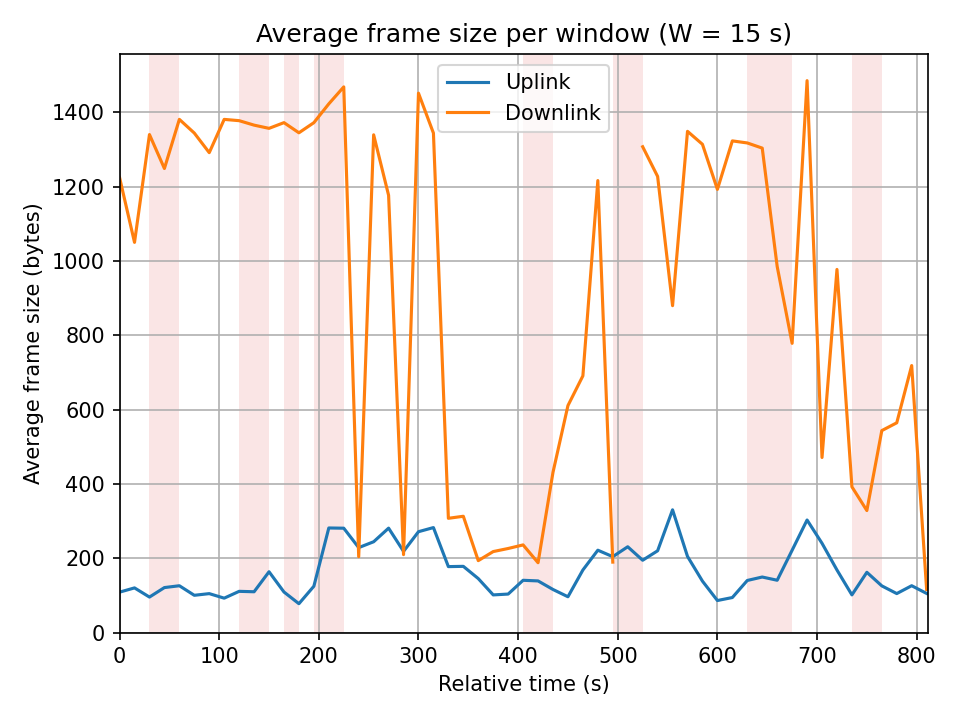
\includegraphics[width=.3\textwidth]{img/plot_frame_size_avg_W15.png}
    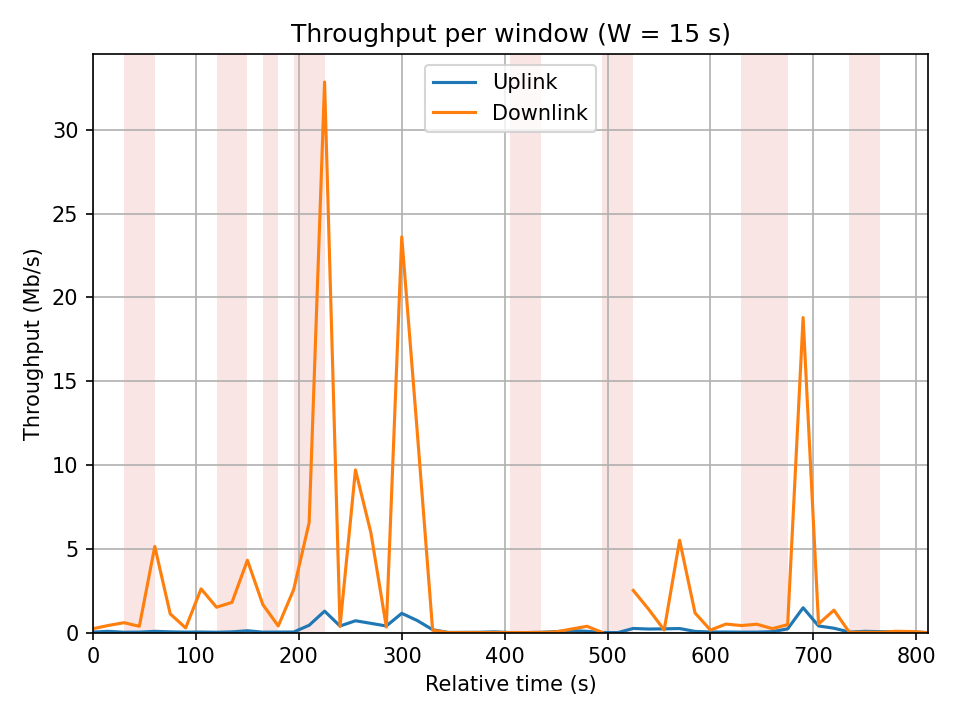
\includegraphics[width=.3\textwidth]{img/plot_throughput_W15.png}
\end{center}
Starting the analysis from frames per second, frame size, and their obvious consequence, throughput:
\begin{itemize}
    \item \textbf{\textit{Average frame size:}} Downlink frames are generally much larger than uplink ones, with consistent sizes above 1,000 bytes during high-traffic periods, while uplink traffic remains small and stable.
    \item \textbf{\textit{Frames per second:}} Strong peaks appear during active downlink traffic, especially when the station is awake. During sleep intervals (red shaded areas), the number of frames drops sharply, confirming reduced channel activity.
    \item \textbf{\textit{Throughput:}} Traffic is heavily dominated by downlink, with bursts up to ~30 Mb/s in short intervals. During sleep phases, throughput collapses close to zero, showing the strong impact of power-saving states on data transfer.
\end{itemize}


\subsubsection*{Inter arrival times}
The plots above show the average and variance of inter-arrival times for uplink and downlink traffic.
\begin{itemize}
    \item Both metrics are generally close to zero, indicating regular packet flows.
    \item Occasional spikes (around 350–400s) correspond to bursts of inactivity followed by traffic resumption, which cause higher inter-arrival times and larger variance.
    \item During predominantly sleeping periods, inter-arrival times remain low, as the station transmits very few packets.
\end{itemize}
These metrics highlight the difference between steady high-throughput traffic and sporadic or bursty transmissions.

\begin{center}
    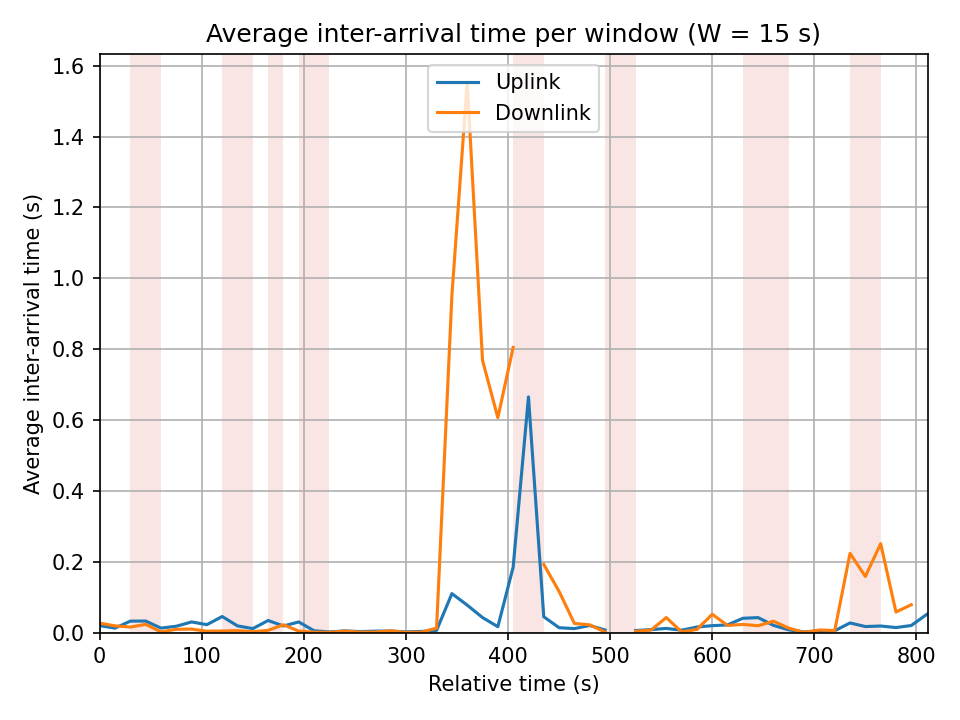
\includegraphics[width=.4\textwidth]{img/plot_iat_avg_W15.png}
    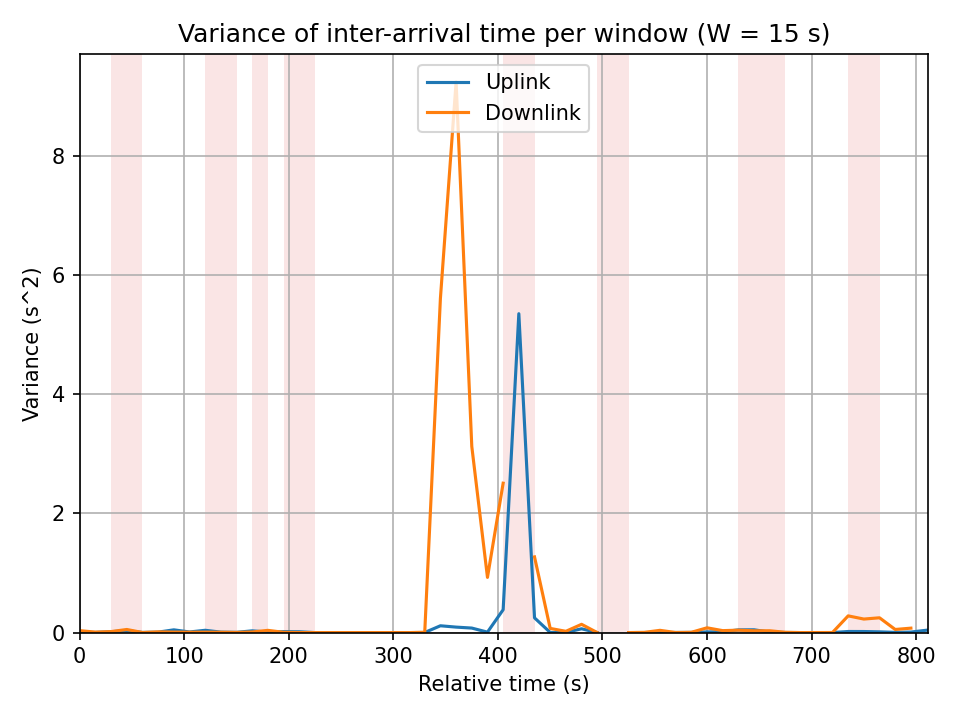
\includegraphics[width=.4\textwidth]{img/plot_iat_var_W15.png}
\end{center}

\subsubsection*{Quality of Service}
The plot illustrates the distribution of QoS access categories over time.
\begin{itemize}
    \item Best Effort (blue) dominates most of the capture, representing general web traffic.
    \item Short intervals of Voice (red) and Video (orange) appear during higher activity phases (e.g., streaming), highlighting latency-sensitive traffic.
    \item Background (green) traffic is sporadic and accounts for only small fractions.
    \item The station tends to enter sleep states during Video traffic, while it almost never sleeps when Best Effort dominates.
\end{itemize}

\begin{center}
    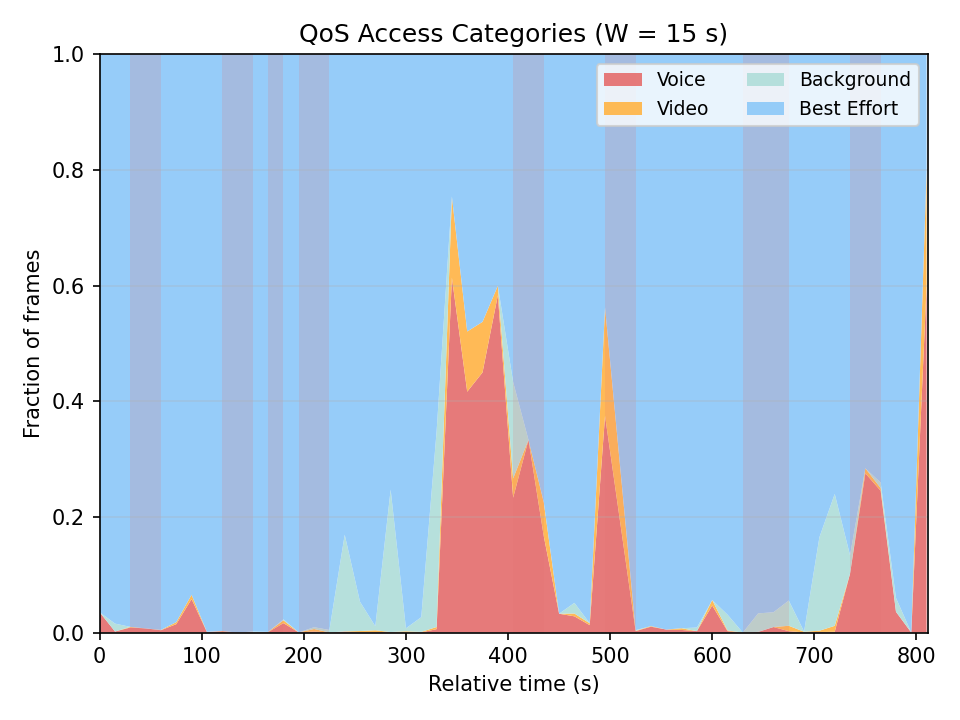
\includegraphics[width=.4\textwidth]{img/plot_qos_composition_W15.png}
\end{center}

\subsubsection*{Random Forest Output}
\begin{lstlisting}
Train acc: 1.0
Test  acc: 0.5454545454545454

accuracy                               0.55        22
macro avg          0.42      0.59      0.48        22
weighted avg       0.39      0.55      0.45        22
\end{lstlisting}

The Random Forest achieved 100\% training accuracy but only ~55\% accuracy on the test set. This indicates clear overfitting: the model memorized the training data but generalized poorly. The classification report also shows that some classes are rarely predicted, confirming class imbalance.\\
This result could be improved by collecting more balanced data across all activities.

\subsubsection*{Confusion Matrix}
The confusion matrix shows that the model is able to clearly distinguish streaming and speedtest sessions, which are recognized with high accuracy. 

\begin{center}
    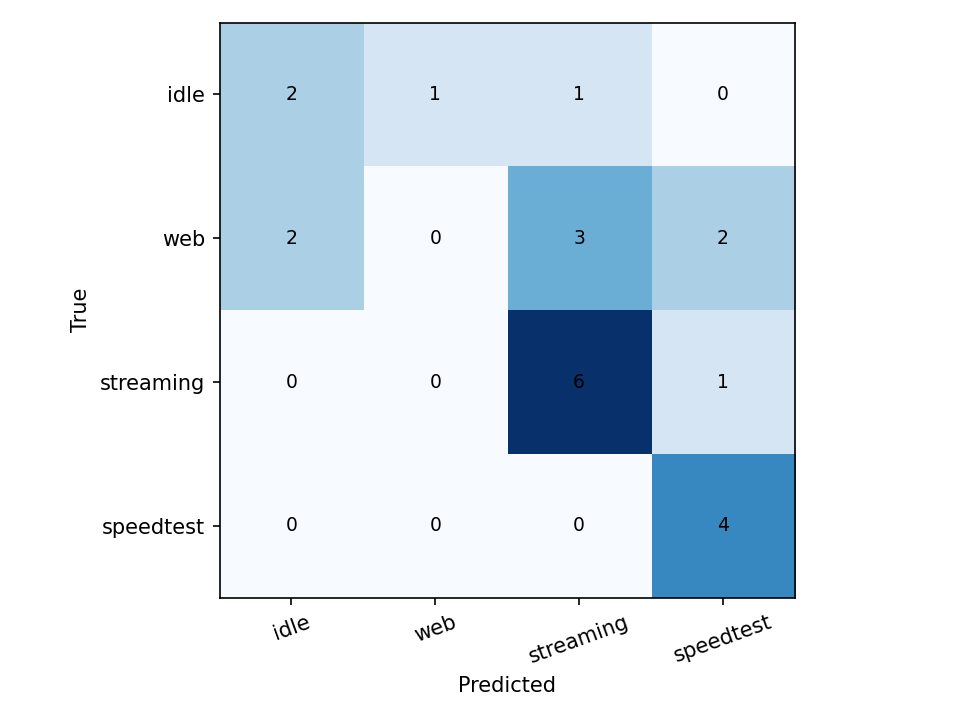
\includegraphics[width=.4\textwidth]{img/confusion_matrix_W15.png}
\end{center}

Web browsing and idle, on the other hand, present more overlap: some idle intervals are misclassified as web or streaming, and part of the web traffic is confused with both streaming and idle.
This outcome reflects the similarity of their traffic patterns, while more distinct behaviors like speedtest (high throughput bursts) and streaming (steady video flows) are easier to separate.


\end{document}